\section{水方halfhda速度6未来发展}
\subsection{已知问题}
本模板未采用2013版规范的页边距设置,因为实在是办不到2.5CM顶部页边距加上2.6CM的页眉设置啊。
\subsection{未来发展}
武汉理工大学本科生论文的未来发展还是需\cite{MartinDSP00}要各位用户的参与,如果每一个用户都能贡献出一点关于\LaTeX 模板的想法和意见,我相信几年之后武汉理工大学本科生论文模板会成为其他高校学习和借鉴的例子。同学当自强,让我们一起来丰富完善这个模板,如果你有很好的建议或者意见请发送到 thesis@tsaoyu.com
\subsection{官方认证}
到目前为止(\today )没有武汉理工大学任何官方组织\cite{吴昉张页-222}对于本模板的格式或者内容进行认证,这代表采用本模板进行的论文写作可能不被官方的论文系统接受。如在进行原创性(防抄袭)检测的时候,可能需要提供提供doc版本的论文。希望用户了解到这个潜在的风险,做好文件转换和备份的准备。本人不对任何由于使用本模板而导致的毕业论文纠纷承担任何责任!
\subsection{测试代码}
%%   插入表格
%%   \hline                            表示横线
%%   \\                                表示换行
%%   \begin{center}   \end{center}     表示表格居中
%%   \centering                        表示表格居中
%%    [!h]    [H]                         固定表格位置
%% 	  \caption{}                       表格自动标号
%%选中若干表格
\begin{table}[H]
\begin{center}
\begin{tabu}{|c|c|c|c|c|}
\hline
foo & foo & foo & foo & foo \\
\hline
foo & foo & foo & foo & foo \\
\hline
foo & foo & foo & foo & foo \\
\hline
\tikzbox{foo} & {foo} &{foo} & {foo} & \tikzbox{foo} \\
\hline
foo & foo & foo & foo & foo \\
\hline
foo & foo & foo & foo & foo \\
\hline
foo & foo & foo & foo & foo \\
\hline
\tikzbox{foo} & \tikzbox{foo} & \tikzbox{foo} & \tikzbox{foo} & \tikzbox{foo} \\
\hline
\end{tabu}
\end{center}
\end{table}

%%两个并列的表格,连在一起写即可(比较窄的表格)
\begin{table}[H]
\begin{center}
\noindent\begin{tabular}{*{3}{c}}
\hline
Header1 & Header 2 & Header3 \\
\hline
Column1a & Column2a & Column3a \\
Column1b & Column2b & Column3b \\
Column1c & Column2c & Column3c \\
Column1d & Column2d & Column3d \\
\hline
\end{tabular}\quad           %% 两个表格的分界线
\begin{tabular}{*{3}{c}}
\toprule
Header1 & Header 2 & Header3 \\
\midrule[2pt]
Column1a & Column2a & Column3a \\
Column1b & Column2b & Column3b \\
Column1c & Column2c & Column3c \\
Column1d & Column2d & Column3d \\
\bottomrule
\end{tabular}
\end{center}
\end{table}

%%一般意义的正常表,表格自动标号\caption{}
\begin{table}[H]       %%表格插入到当前位置【h】,【!】表示不考虑美学
\caption{kdjakjdfkajd}  %%caption内部是表格的题注
\centering
\begin{tabular}{cc}
\toprule
Header1 & Header 2 \\
\midrule[2pt]
Column1a & Column2a  \\
Column1b & Column2b  \\
Column1c & Column2c \\
Column1d & Column2d \\
\bottomrule
\end{tabular}
\end{table}

%%具有行列合并的表格
%%建议先复制这段代码跑出表格,然后分析代码
\begin{table}[H]   %%【htb】,表格插入到here,top或者bottom
\caption{kdjakjdfkajd}
\centering
\begin{tabular}{c|cc}
\toprule
Header1 & Header2 & Header3 \\
\midrule[2pt]
\multicolumn{3}{c}{\textbf{Column1a} } \\             %行合并(合并第一行)
Column1b & Column2b & \multirow{3}{*}{\tabincell{c}{the first line \\ the next}} \\     %%列合并
Column1c & Column2c \\
Column1d & Column2d &  \\
\bottomrule
\end{tabular}
\end{table}

%% 美赛表格汇总
%%变量表
\begin{table}[H]
\caption{Symbol Table-Variables1}
\centering
\begin{tabular}{lll}
\toprule
Symbol & Definition  & Units\\
\midrule[2pt]
\multicolumn{3}{c}{\textbf{Variables} }\\
\multirow{3}{*}{\tabincell{l}{  $N$  } }& \multirow{3}{*}{\tabincell{l}{the first lineThe number of vehicles\\ passing a certain point on the highway } } & \multirow{3}{*}{\tabincell{l}{ unitless} }  \\
\\
\\
$L$ & Lenth of cell & cell   \\
${c_i}$ & The serial number of cell (Number i)   & unitless\\
$({r_i},{c_i})$ & the position of cell(Number i) & unitless\\
${r_{i}}$ & The serial number of Lane(Number i) & unitless\\
${r_{ti}}$ & The serial number of Target Lane(Number i) & unitless\\
$Head({r_i},{c_i})$ &Front gap  & cell\\
${Head_{side}}({r_i},{c_i})$ & Side front gap & cell\\
$Back({r_i},{c_i})$ & Back gap  & cell\\
${Back_{side}}({r_i},{c_i})$ &Side back gap  & cell\\
${v_i}$ &  The current speed of car(Number i)& cell/time-step\\
${v_{ti}}$ &The target speed of car(Number i)  & cell/time-step\\


\bottomrule
\end{tabular}
\end{table}
%%----------------------------------------------
\begin{table}[H]
\caption{Symbol Table-Variables2}
\centering
\begin{tabular}{lll}
\toprule
Symbol & Definition  & Units\\
\midrule[2pt]
${v_{limit}}$ &Maximum speed limit  & cell/time-step\\
$ v_{mean}$ &Average speed&  cell/time-step \\
${{\bar v_i}}$ &  Average speed(Number i)& cell/time-step\\
${p_{brake}}$ &  Probability of Accidental braking & unitless\\
${p_{Lc}}$ & Probability of Lane-Changing & unitless\\
${\theta }$ &The percentage of self-driving car  & unitless\\
${\tau }$ & Friendliness coefficient & unitless\\
${ \delta}$ & The extent of the back car affected & unitless\\
$\lambda$  & Expectancy of poisson-distribution & unitless  \\
${l_{a,safe}}$ &Safe distance of self-driving-car& cell\\
${l_{n,safe}}$ &Safe distance of None-self-driving car& cell\\
\multirow{2}{*}{\tabincell{l}{  $NL$  } }& \multirow{2}{*}{\tabincell{l}{the number of lanes } } & \multirow{2}{*}{\tabincell{l}{ unitless} }  \\
\\
$\Omega  $ & Lane changing algorithm & unitless\\
$\xi$  &Traffic flow over a period of time &  cell \\
${\xi _d}$&Average daily traffic volume& cell \\
${\xi _p}$&Traffic flow during peak hours& cell \\
$T$ &Iteration time& time-step\\
$t$&Iterative time slot & time-step\\
$DL$ & the number of dedicated lane&  unitless \\
$ L_{safe}$  & Average safe distance &  cell \\
$ L_{average}$  &Average vehicle length &  cell \\
$\eta$ &Average vehicle flow efficiency& unitless \\ 
\bottomrule
\end{tabular}
\end{table}
%%----------------------------------------------
\begin{table}[!h]
\caption{ Detailed configuration}
\centering
\begin{tabular}{ll|ll}
\toprule
Index &  value  & Index & value\\
\midrule[2pt]
$NL$ & 1/2/3   &$\theta $     & [0,1]\\
$L$ & 1000cell    &$\lambda  $    &\{0.1,0.25,0.5,10\} \\
$\tau$ &[0,1]   &${v_{limit}}$  &  10cell/time-step\\
 \multirow{2}{*}{\tabincell{c}{$\Omega  $}}  &  \multirow{2}{*}{\tabincell{c}{CCL/NCL/ACL/\\FCL}}&  $DL$  &  0/1/2/3  \\
 \\
\bottomrule
\end{tabular}
\end{table}
%%----------------------------------------------
\begin{table}[H]
\caption{ 中文表}
\centering
\begin{tabular}{ll|ll}
\toprule
项目 &  取值  &项目 & 取值\\
\midrule[2pt]
$NL$ & 1/2/3   &$\theta $     & [0,1]\\
$L$ & 1000cell    &$\lambda  $    &\{0.1,0.25,0.5,10\} \\
$\tau$ &[0,1]   &${v_{limit}}$  &  10cell/time-step\\
 \multirow{2}{*}{\tabincell{c}{$\Omega  $}}  &  \multirow{2}{*}{\tabincell{c}{CCL/NCL/ACL/\\FCL}}&  $DL$  &  0/1/2/3  \\
 \\
\bottomrule
\end{tabular}
\end{table}

%%单独一个图片
\begin{figure}[H]
\small
\centering
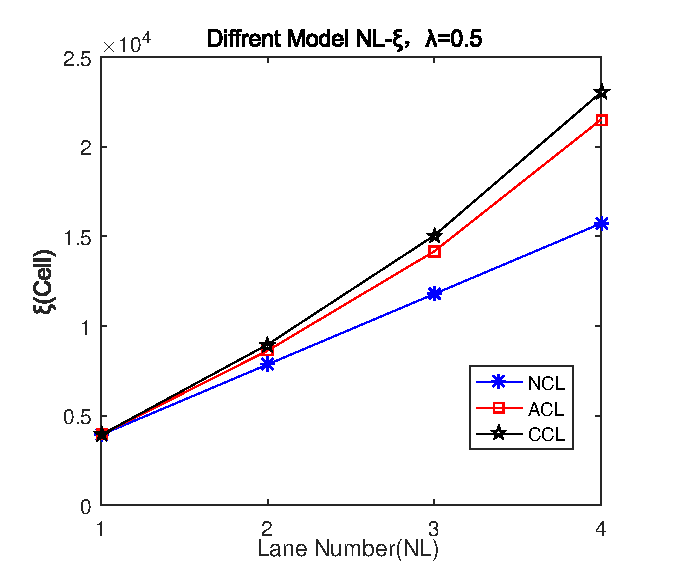
\includegraphics[width=8cm]{figure/421.eps}
\caption{a picture} \label{fig:a picture}
\end{figure}

%%插入两个并列图片4221和4222
\begin{figure}[H]
\centering
\subfigure[None dedicated lane]{
\label{figa} %% label for first subfigure
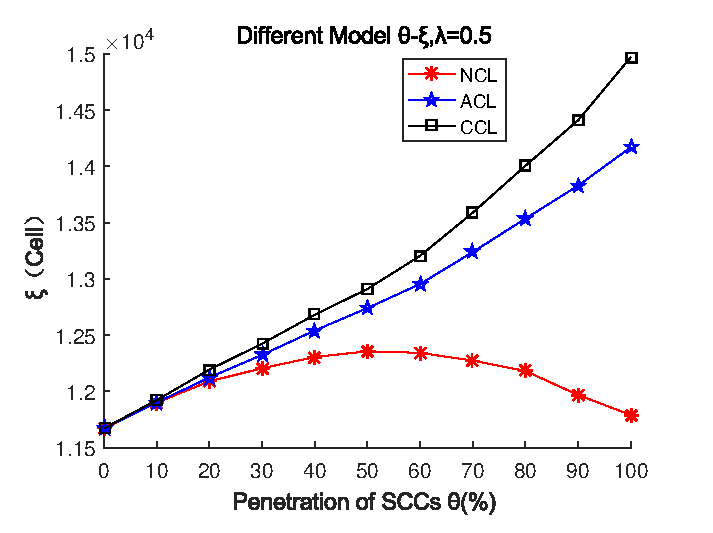
\includegraphics[width=5.3cm]{figure/4221.eps}}
\hspace{0cm}
\subfigure[Dedicated lane]{
\label{fig:subfig:b} %% label for second subfigure
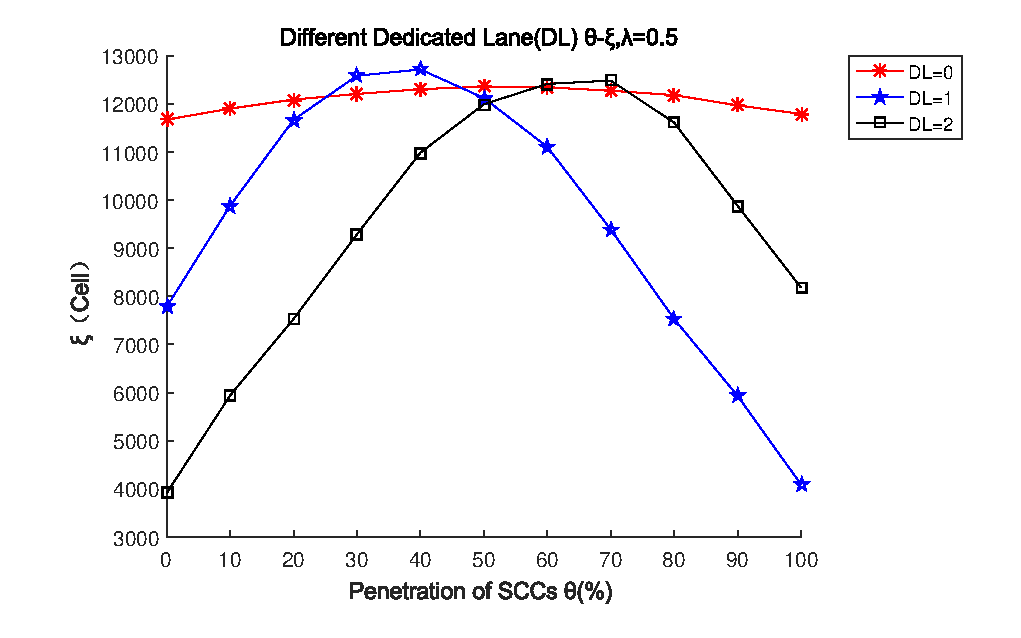
\includegraphics[width=6.6cm]{figure/4222.eps}}
\caption{Simulation Results for NCL,ACL,and CCL}
\label{figb} %% label for entire figure
\end{figure}


%%以下为定理代码
\begin{Theorem} 
for i>0, i++.
\end{Theorem}

%%以下为引理代码
\begin{Lemma} 
\TeX .
\end{Lemma}

\begin{Lemma} 
\TeX .
\end{Lemma}

\begin{Lemma} 
\TeX .
\end{Lemma}

\begin{Theorem} 
for i>0, i++.
\end{Theorem}

%%以下为证明
\begin{proof}
The proof of theorem.
\end{proof}

%%不一定要会,因为可以用mathtype写出公式之后导出latex代码
%%但是有时mathtype的公式导出时会出bug
%%所以建议还是看一看


%%公式输入,熟悉角标即可(常用)
%%    \]   和  $$  都是无编号的公式输入
%%      \begin{equation}  是有编号的输入
\begin{equation}
\sum\limits_{i = 1}^n {X_i^2} \sum\limits_{i = 1}^n {{X_i}{Y_i}} \frac{1}{n}\sum\limits_{i = 1}^n {{{({X_i} - \bar X)}^2}}       
\end{equation}

%%左对齐连续等号
\begin{equation}
\begin{array}{lllll}
 & \frac{{\delta y}}{{\delta x}}\\
{\rm{ = }} & \mathop {\lim }\limits_{\delta x \to 0} \\
{\rm{ = }} & \sum\limits_{i = 1}^n {{X_i}{Y_i}} \oint_S x dx\\
{\rm{ = }} & \sum\limits_{i = 1}^n {{{({X_i} - \bar X)}^2}} 
\end{array}
\end{equation}           %% 带上标号

%%矩阵
\[\left( {\begin{array}{*{20}{c}}
{{a_1}}&{}&0\\
{}& \ddots &{}\\
0&{}&{{a_n}}
\end{array}} \right)\left( {\begin{array}{*{20}{c}}
1&0\\
0&1
\end{array}} \right)\left( {\begin{array}{*{20}{c}}
{{a_{11}}}& \ldots &{{a_{1n}}}\\
 \vdots & \ddots & \vdots \\
{{a_{m1}}}& \cdots &{{a_{mn}}}
\end{array}} \right)\]


%%大括号分类
\[\left\{ \begin{array}{l}
ad\\
adf\\
adfa
\end{array} \right.\]

\begin{equation}
{p_{Lc,i}} = f({\delta _j},\tau ) = \left\{ \begin{array}{l}
1    ,{\delta _j} = 0\\
0   , {\delta _j} = 1\\
\max ( - \frac{\tau }{{1 - \tau }} \cdot {\delta _j} + 1,0){\rm{     }},otherwise{\rm{ }}
\end{array} \right.
\end{equation} 


\begin{equation}
{P_t}(n) = \frac{{{\lambda ^n}}}{{n!}}{e^{ - \lambda }}(n > 0)
\end{equation}
The $\lambda$ indicates the number of vehicles per unit time t. Let $ \lambda = \alpha t $, and $\alpha$ represents the average arrival rate of the vehicle. The Poisson distribution formula $(4.1)$ can be transformed into:
 \begin{equation}
{p_n}(t) = \frac{{{{(\alpha t)}^n}}}{{n!}}{e^{ - \alpha t}}(t > 0)
\end{equation}

%%无序列举
\begin{itemize}
\item  我的号哈佛的
\item  马上量很大
\item  撒考核法开始的恢复
\end{itemize}


%%加粗列举(看起来会很赞)
\begin{itemize}
\item \textbf{好的卡焦点科技几点开始}
\item \textbf{阿发达}
\item \textbf{看了就烦对哦}
\end{itemize}